\documentclass{beamer}
\usepackage[utf8]{inputenc}
\usepackage{ragged2e}
\usepackage{graphicx}
\usepackage{caption}
\usepackage{placeins}
\usepackage{todonotes}
\usepackage{subcaption}
\usepackage[font=footnotesize,labelformat=simple]{subcaption}

\usetheme{Madrid}
\usecolortheme{default}

%------------------------------------------------------------
%This block of code defines the information to appear in the
%Title page
\title[Slide deck - Colombia] %optional
{Slide deck - Colombia}

\subtitle{Proposed outline}

\author{Nathalie Gonzalez-Prieto} % (optional)

\institute{World Bank} % (optional)


\date[WB 2024] % (optional)
{Conference, December 2024}


%End of title page configuration block
%------------------------------------------------------------



%------------------------------------------------------------
%The next block of commands puts the table of contents at the 
%beginning of each section and highlights the current section:

\AtBeginSection[]
{
  \begin{frame}
    \frametitle{Table of Contents}
    \tableofcontents[currentsection]
  \end{frame}
}
%------------------------------------------------------------


\begin{document}

%The next statement creates the title page.
\frame{\titlepage}


%---------------------------------------------------------
%This block of code is for the table of contents after
%the title page
\begin{frame}
\frametitle{Table of Contents}
\tableofcontents
\end{frame}
%---------------------------------------------------------


\section{Changes over time}

%---------------------------------------------------------

\begin{frame}
\frametitle{Changes over time}
\begin{figure}[!htb]
    \justifying
     \caption{Workers who do not contribute to SS}     
     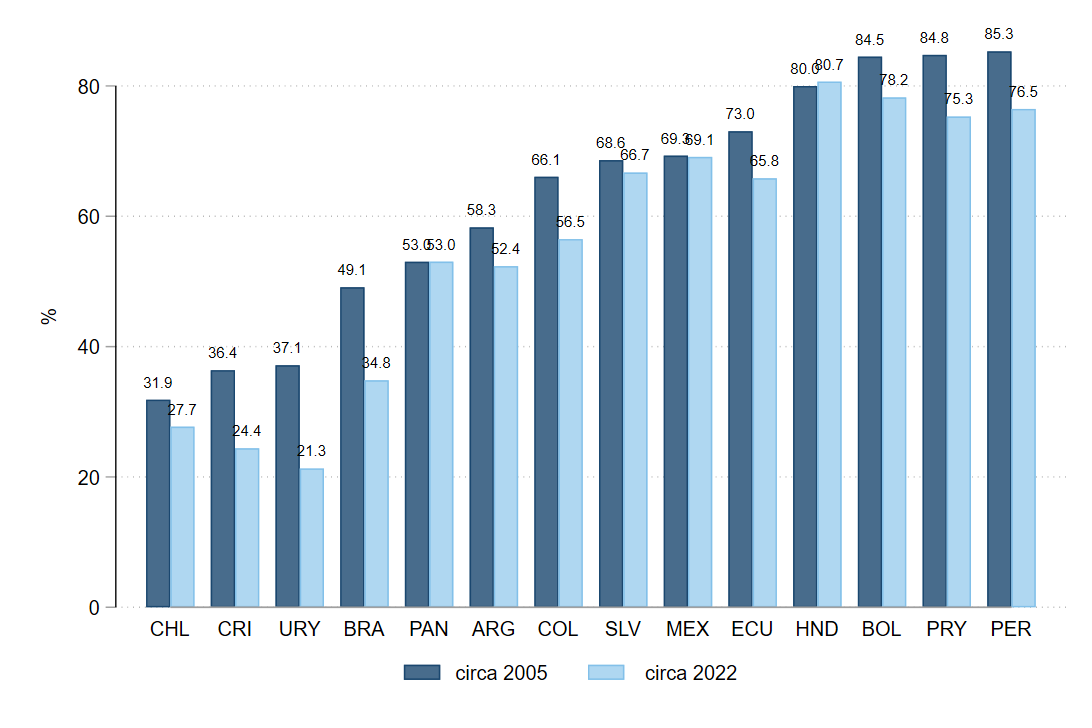
\includegraphics[width=0.5\linewidth]{latex/figures/Snapshot/snapshot_informal_ss.png}
    \label{fig:SalariedSS}
    \footnotesize{Source: Household Surveys-SEDLAC.}
    \footnotesize{Note: Each bar is a weighted average of each country, weighting by total workers in 2005 and 2021.  Data corresponds to 2021 except for Chile 2022, Guatemala 2014; Honduras 2019; Mexico 2018 and Uruguay 2019.}
\end{figure}
    
\end{frame}

%---------------------------------------------------------
%---------------------------------------------------------

\begin{frame}
\frametitle{Changes over time}
\begin{figure}[!htb]
    \justifying
     \caption{Workers who work at small firms}     
     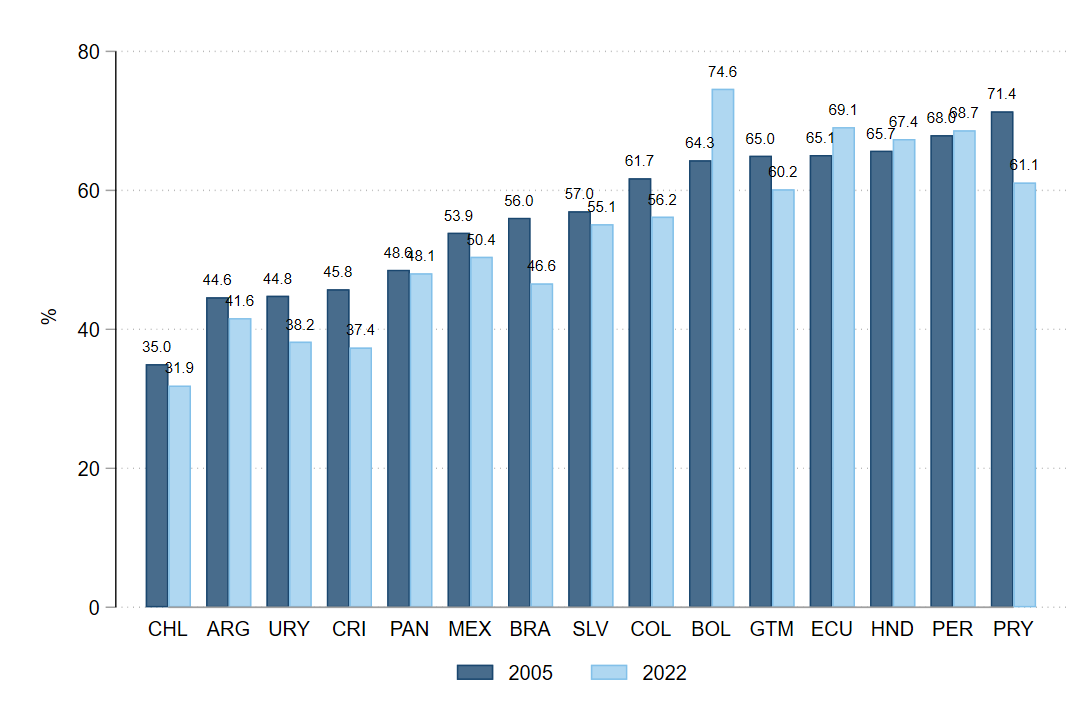
\includegraphics[width=0.5\linewidth]{latex/figures/Snapshot/snapshot_workers_small.png}
    \label{fig:SalariedSmall}
    \footnotesize{Source: Household Surveys-SEDLAC.}
    \footnotesize{Note: Each bar is a weighted average of each country, weighting by total workers in 2005 and 2021.  Data corresponds to 2021 except for Chile 2022, Guatemala 2014; Honduras 2019; Mexico 2018 and Uruguay 2019.}
\end{figure}
\end{frame}
%---------------------------------------------------------
%---------------------------------------------------------

\begin{frame}
\frametitle{Changes over time}
\begin{figure}[!htb]
    \justifying
     \caption{Salaried who do not contribute to SS}     
       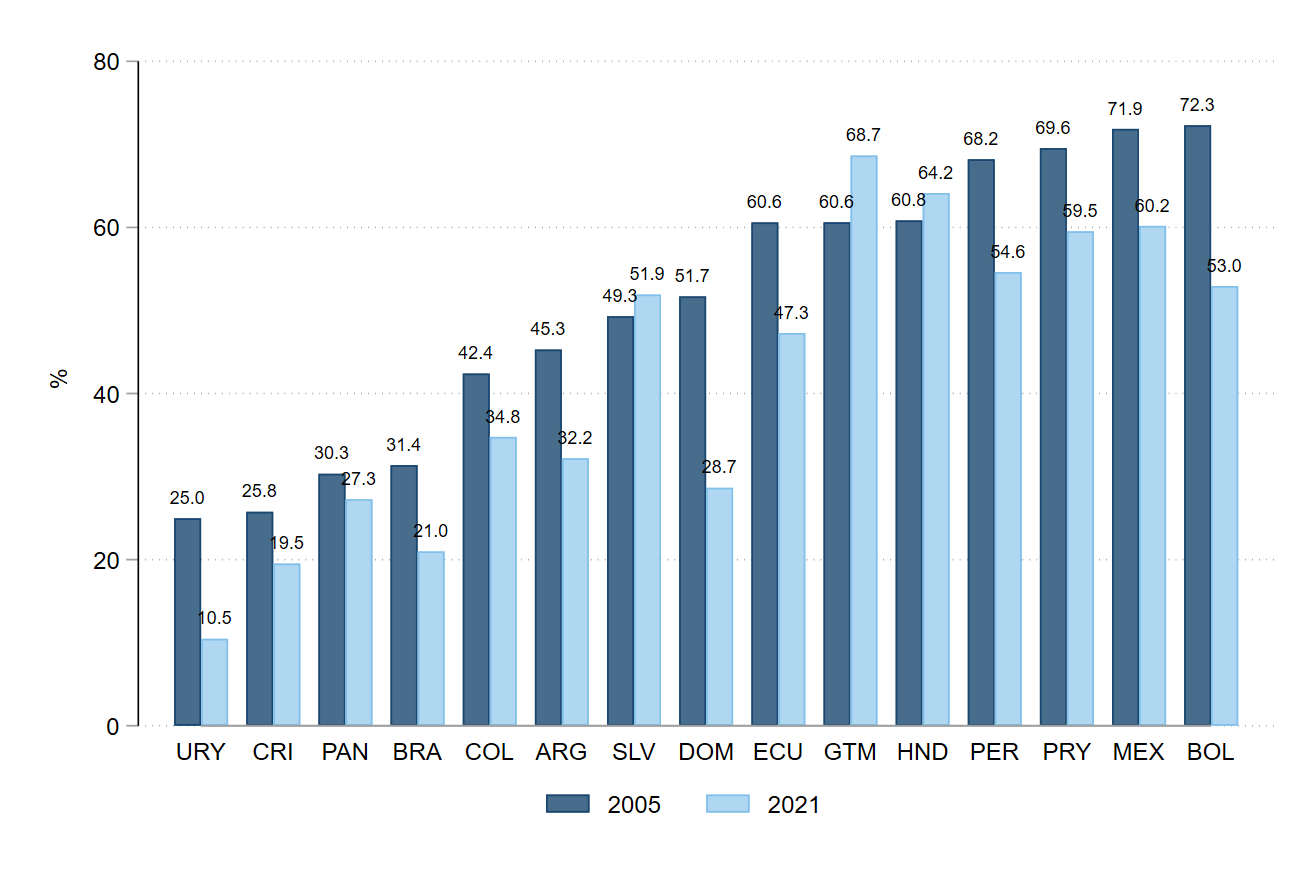
\includegraphics[width=0.5\linewidth]
       {latex/figures/Snapshot/snapshot_informal_ss_dep.png}
    \label{fig:SalariedSS}
    \footnotesize{Source: Household Surveys-SEDLAC.}
    \footnotesize{Note: Each bar is a weighted average of each country, weighting by total workers in 2005 and 2021.  Data corresponds to 2021 except for Chile 2022, Guatemala 2014; Honduras 2019; Mexico 2018 and Uruguay 2019.}
\end{figure}


    
\end{frame}

%---------------------------------------------------------
%---------------------------------------------------------

\begin{frame}
\frametitle{Changes over time}
\begin{figure}[!htb]
    \justifying
     \caption{Salaried who work at small firms}     
     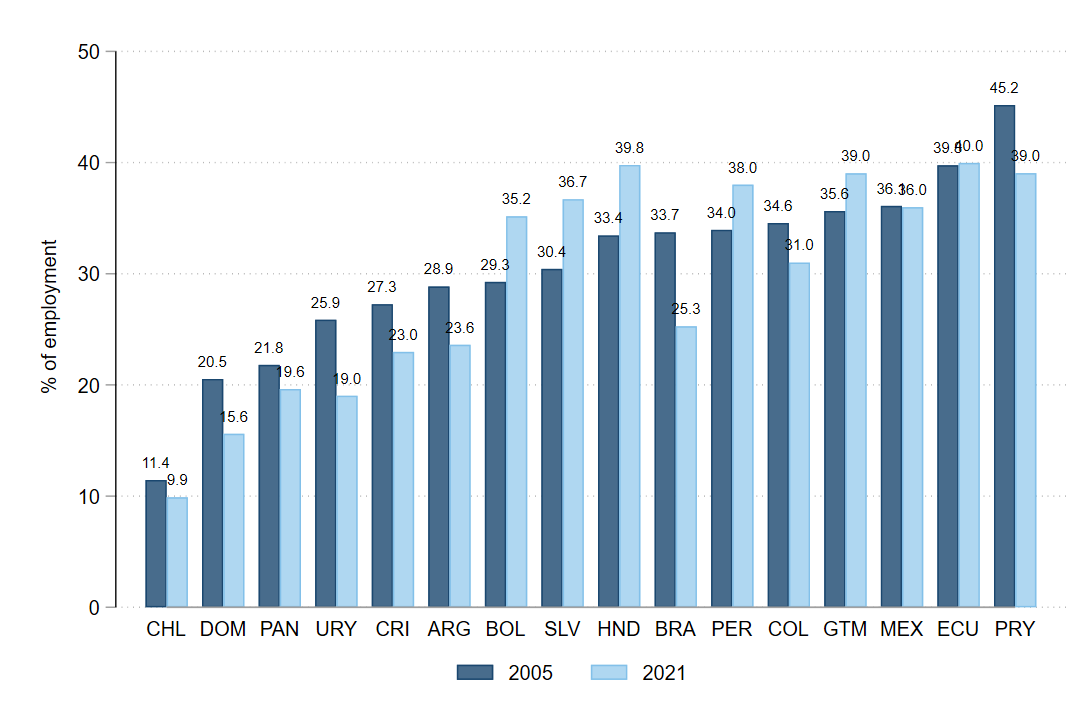
\includegraphics[width=0.5\linewidth]{latex/figures/Snapshot/snapshot_dependents_small.png}
    \label{fig:SalariedSmall}
    \footnotesize{Source: Household Surveys-SEDLAC.}
    \footnotesize{Note: Each bar is a weighted average of each country, weighting by total workers in 2005 and 2021.  Data corresponds to 2021 except for Chile 2022, Guatemala 2014; Honduras 2019; Mexico 2018 and Uruguay 2019.}
\end{figure}
\end{frame}
%---------------------------------------------------------

%---------------------------------------------------------

\section{Regional heterogeneity}

%---------------------------------------------------------
%---------------------------------------------------------

\begin{frame}
\frametitle{Regional heterogeneity}
\begin{figure}[!htb]
\justifying
  \caption{Demographic profile and structure of labor market}
\begin{subfigure}{.9\textwidth}
  \centering
    \subcaption{Demographic}
  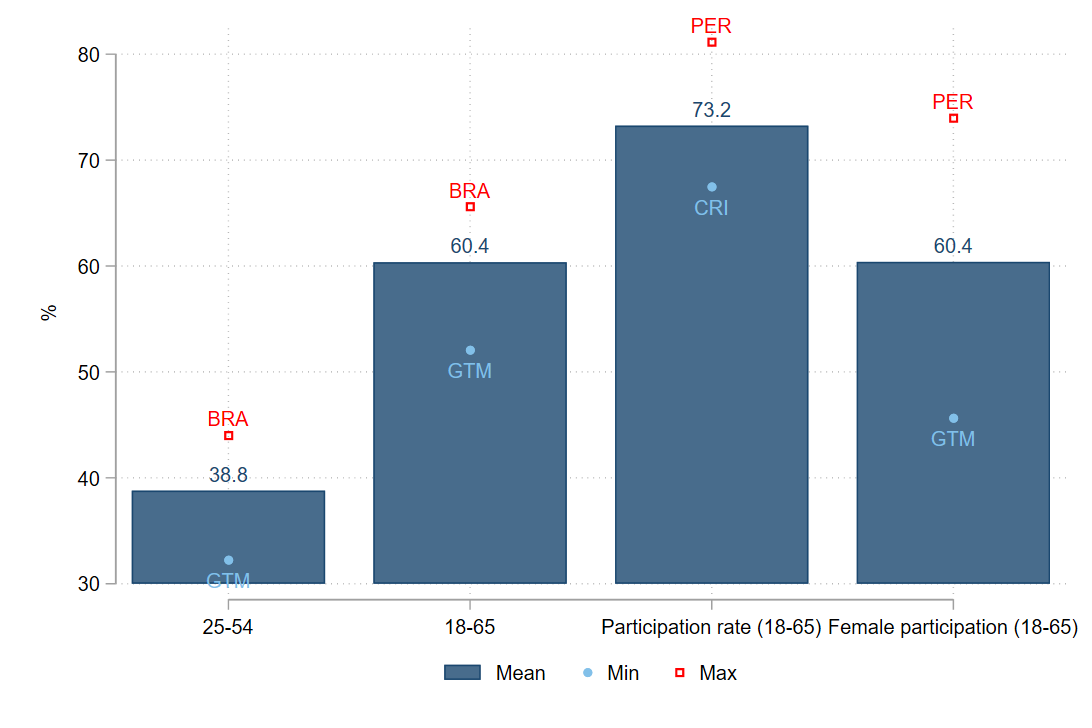
\includegraphics[width=0.5\linewidth]{latex/figures/Snapshot/Structure of labor market_a.png}
  \label{fig:labmarket1}
\end{subfigure}

\begin{subfigure}{.9\textwidth}
  \centering
    \subcaption{Labor market}
  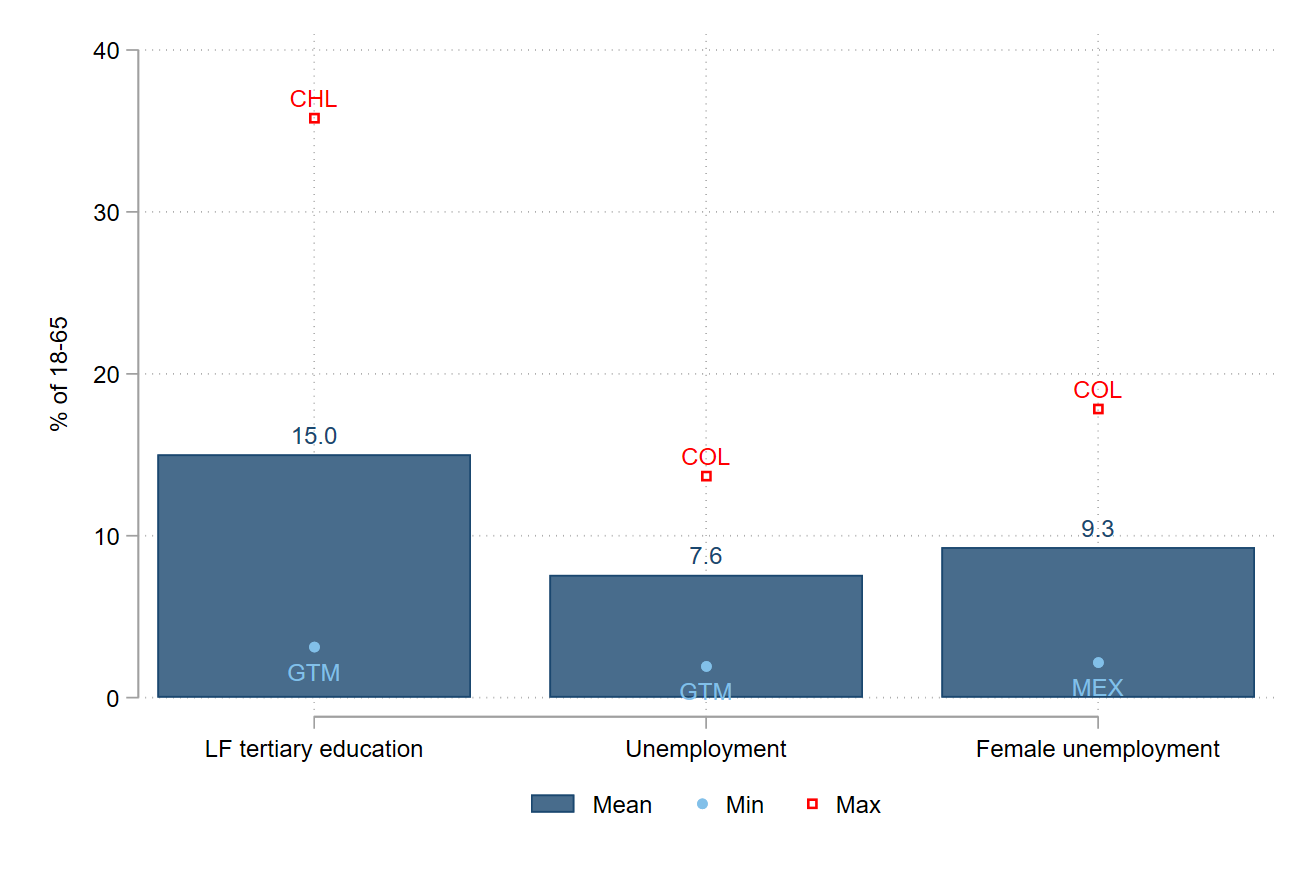
\includegraphics[width=0.5\linewidth]{latex/figures/Snapshot/Structure of labor market_b.png}
  \label{fig:labmarket2}
\end{subfigure}

\footnotesize{Source: Household Surveys-SEDLAC.}
\footnotesize{Note: Each bar is a simple average of country level weighted average in 2021. Countries included in the sample: Argentina, Bolivia, Brazil, Chile, Colombia, Costa Rica, Dominican Republic, Ecuador, El Salvador, Guatemala, Honduras, Mexico, Panama, Peru, Paraguay and Uruguay. Some countries don’t have information for 2021, in that cases we use the last available year, for Chile 2022, Guatemala 2014; Honduras 2019; Mexico 2018 and Uruguay 2019. Panel a: bar one and two are defined as percentage of the population. Also, "Participation rate" and "Female participation" are define as part of the labor force defined for people between 18 and 65 years old. Panel b: "LF tertiary education" corresponds to people in the workforce who have completed tertiary education.}

\end{figure}

\end{frame}
%---------------------------------------------------------

%---------------------------------------------------------
\begin{frame}
\frametitle{Regional heterogeneity}
 \begin{figure}[!htb]
        \justifying
        \caption{Structure of employment}     
        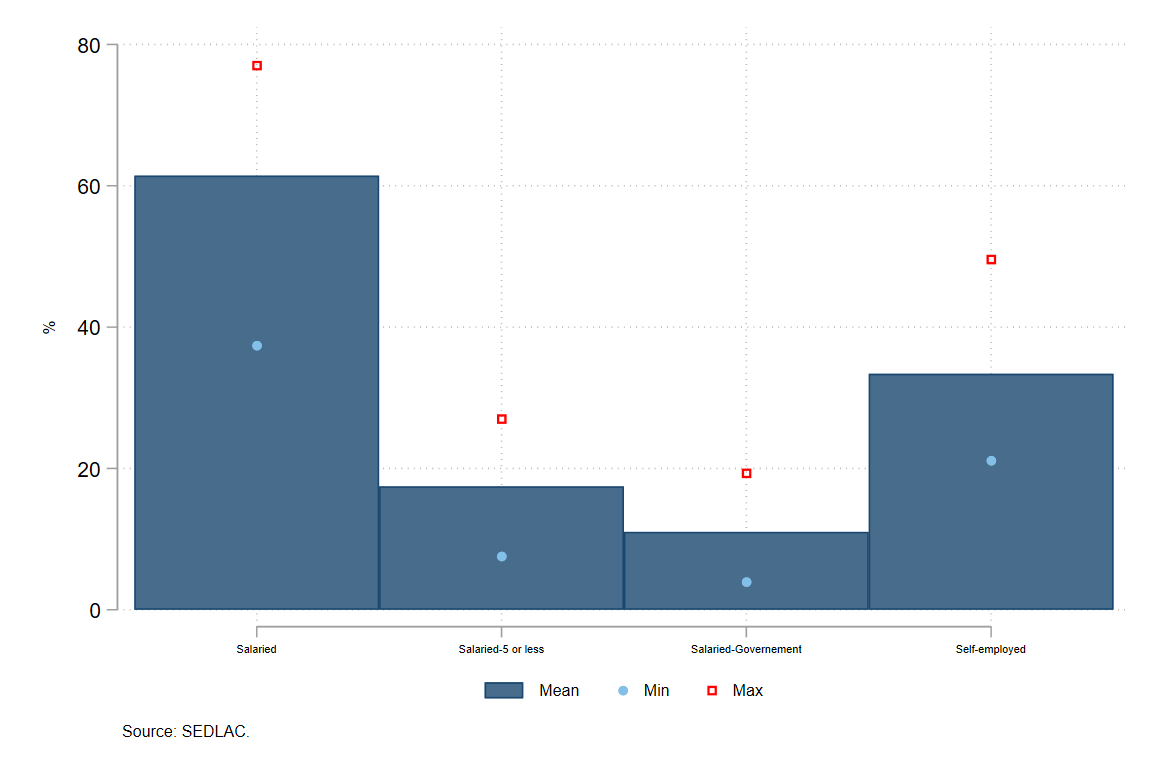
\includegraphics[scale=.2]{latex/figures/Snapshot/Structure of employment.png}
        \label{fig:employment}
        \footnotesize{Source: Household Surveys-SEDLAC.}
        \footnotesize{Note: Each bar is a simple average of country level weighted average in 2021. Countries included in the sample: Argentina, Bolivia, Brazil, Chile, Colombia, Costa Rica, Dominican Republic, Ecuador, El Salvador, Guatemala, Honduras, Mexico, Panama, Peru, Paraguay and Uruguay. Some countries don’t have information for 2021, in that cases we use the last available year, for Chile 2022, Guatemala 2014; Honduras 2019; Mexico 2018 and Uruguay 2019. The "non-salaried" category corresponds to unpaid workers such as family or cooperative workers.}
\end{figure}
\end{frame}
%---------------------------------------------------------
     
%---------------------------------------------------------
\begin{frame}
\frametitle{Regional heterogeneity}
\begin{figure}[!htb]
        \justifying
        \caption{Structure of employment by sector}     
        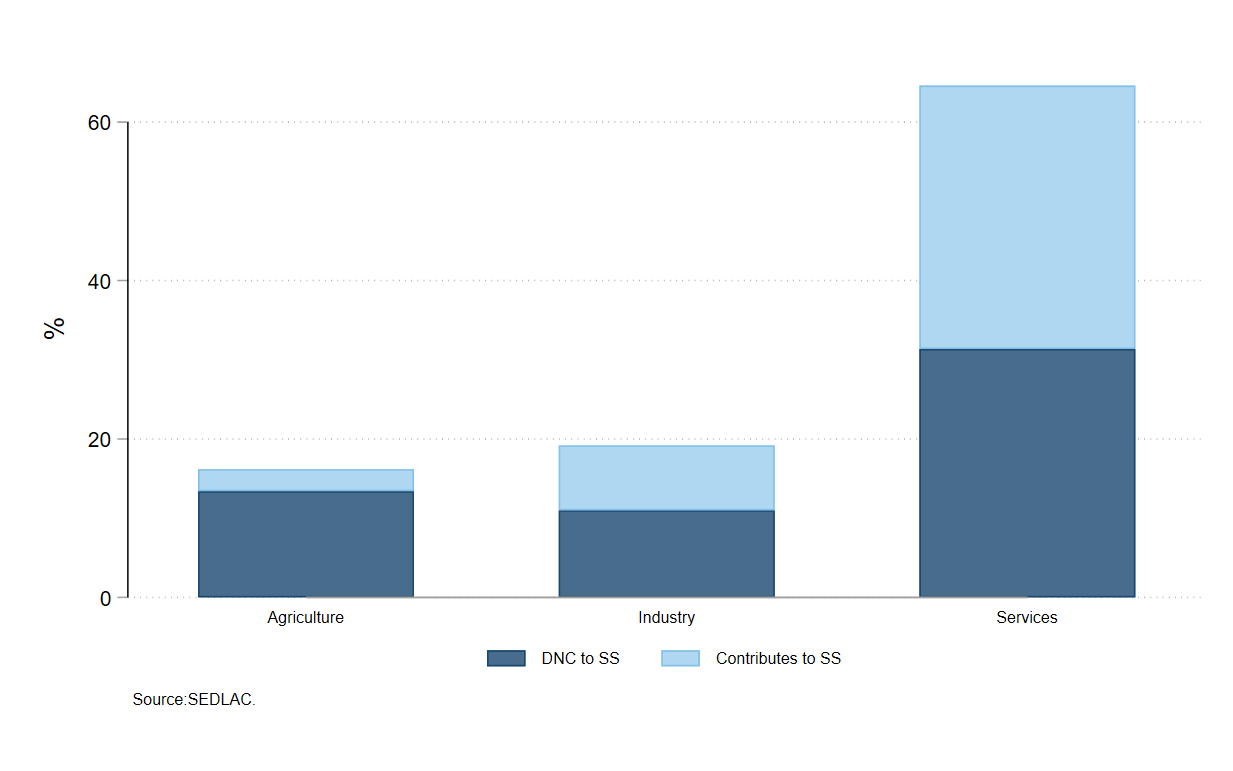
\includegraphics[scale=.2]{latex/figures/Snapshot/Structure of employment and sector.png}
        \label{fig:sector}
       \footnotesize{Source: Household Surveys-SEDLAC.}
        \footnotesize{Note: Each bar is a simple average of country level weighted average in 2021. Countries included in the sample: Bolivia, Brazil, Chile, Colombia, Costa Rica, Dominican Republic, Ecuador, El Salvador, Guatemala, Honduras, Mexico, Panama, Peru, Paraguay and Uruguay. Some countries don’t have information for 2021, in that cases we use the last available year, for Chile 2022, Guatemala 2014; Honduras 2019; Mexico 2018 and Uruguay 2019. Argentina is excluded from this figure because the household survey is urban.}
\end{figure}
\end{frame}
%---------------------------------------------------------

%---------------------------------------------------------
\begin{frame}
\frametitle{Regional heterogeneity}
\begin{figure}[!htb]
        \justifying
        \caption{Structure of private employment by firm size}     
        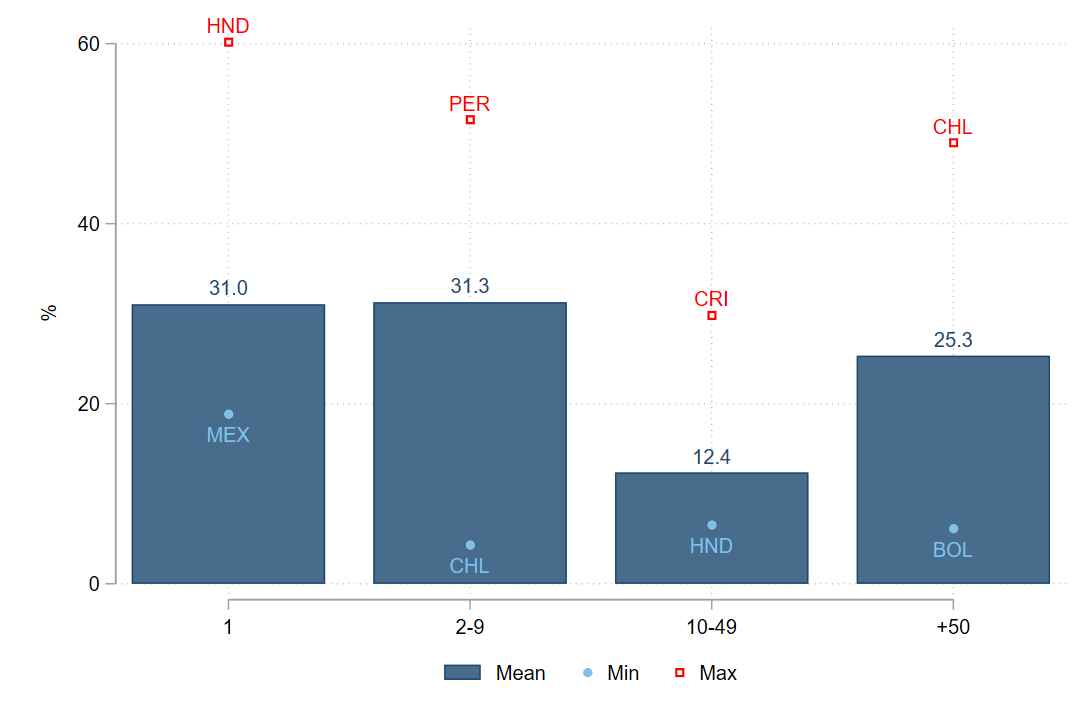
\includegraphics[scale=.2]{latex/figures/Snapshot/Structure of employment by firm size.png}
        \label{fig:firmsize}
        \footnotesize{Source: Household Surveys-SEDLAC.}
        \footnotesize{Note: Each bar is a simple average of country level weighted average in 2021. Countries included in the sample: Bolivia, Brazil, Chile, Colombia, Costa Rica, Ecuador, El Salvador, Honduras, Mexico, Panama, Peru, Paraguay and Uruguay. Some countries don’t have information for 2021, in that cases we use the last available year, for Chile 2022, Guatemala 2014; Honduras 2019; Mexico 2018 and Uruguay 2019. We exclude Argentina, Dominican Republic and Guatemala, because of missing information in firm size variable.}
        \end{figure}

\end{frame}
%---------------------------------------------------------
%---------------------------------------------------------
\begin{frame}
\frametitle{Regional heterogeneity}
\begin{figure}[!htb]
        \justifying
        \caption{Share of Workers Who Do Not Contribute to Social Security by Selected Characteristics}     
        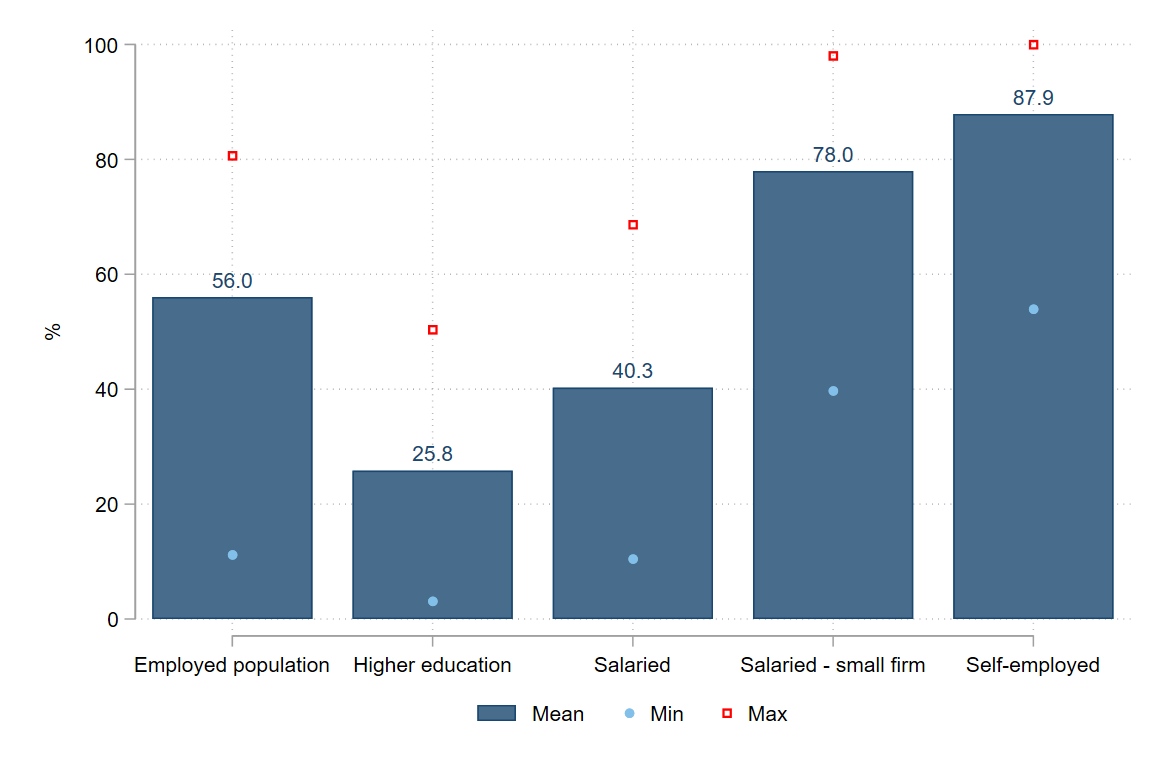
\includegraphics[scale=.2]{latex/figures/Snapshot/Social security contributions.png}
        \label{fig:SScontributions}
        \footnotesize{Source: Household Surveys-SEDLAC.}
        \footnotesize{Note: Each bar is a simple average of country level weighted average in 2021. Countries included in the sample: Argentina, Bolivia, Brazil, Chile, Colombia, Costa Rica, Dominican Republic, Ecuador, El Salvador, Guatemala, Honduras, Mexico, Panama, Peru, Paraguay and Uruguay. Some countries don’t have information for 2021, in that cases we use the last available year, for Chile 2022, Guatemala 2014; Honduras 2019; Mexico 2018 and Uruguay 2019. \textbf{The groups are not exclusive.} "Tertiary education" corresponds to people in the workforce who have completed tertiary level of education. "Salaried-Small firm" are salaried employees that work in a firm of 5 or less workers.}
 \end{figure}
 \end{frame}
%---------------------------------------------------------
%---------------------------------------------------------

\section{Dynamics: last 20 years}  
%---------------------------------------------------------
%---------------------------------------------------------
\begin{frame}
\frametitle{Dynamics: last 20 years}
\begin{figure}[!htb]
        \justifying
        \caption{Evolution of alternative informality related measures}     
        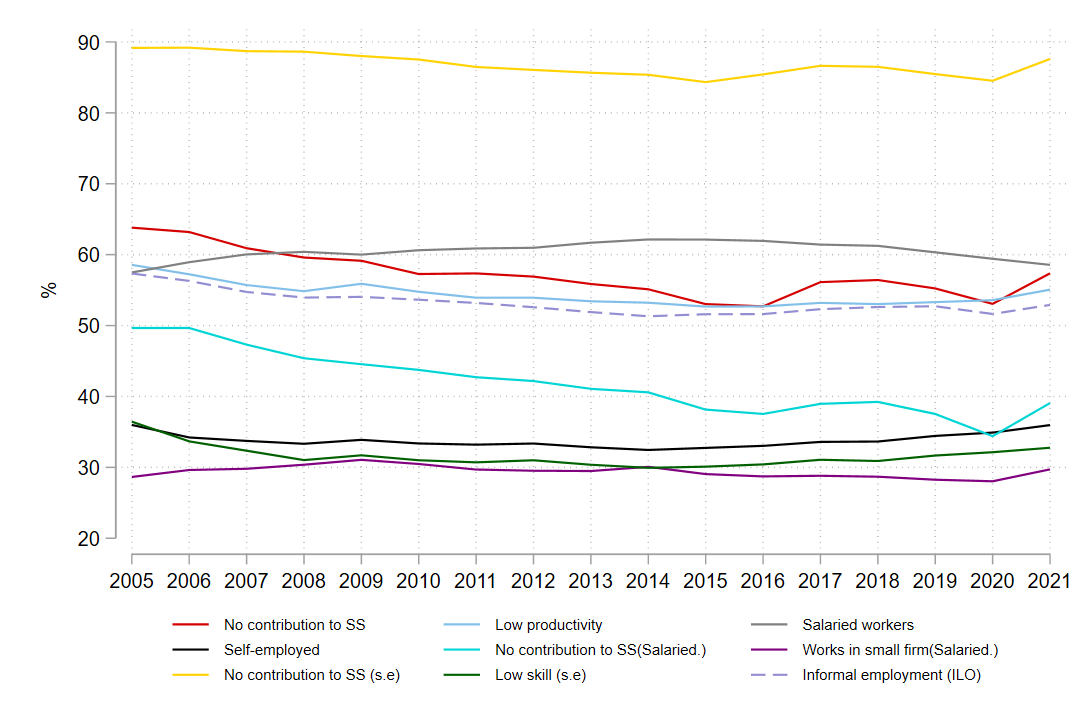
\includegraphics[scale=.2]{latex/figures/Evolution/informality_evolution_LAC.png}
        \label{fig:EvolutionLAC}
        \footnotesize{Source: Household Surveys-SEDLAC and ILO.}
        \footnotesize{Note SEDLAC: The figure shows unweighted means of country level indicators. The countries included in the sample are Argentina, Bolivia, Brazil, Colombia, Costa Rica, Ecuador, Guatemala, Dominican Republic, Honduras, Mexico, Panama, Peru, Paraguay, El Salvador and Uruguay. Some countries don’t have information for the entire period: Bolivia and Brazil have missing values in 2010; Colombia have missing values in 2006 and 2007; Honduras have missing values in 2020-2021; Mexico have missing values 2005, 2007, 2009, 2011, 2013, 2015, 2017, 2019, 2020, 2021; Panama and El Salvador have missing values 2020; and Uruguay have missing values in 2021. Note ILO: The serie is a modeled estimated informal employment rate by ILO.}
 \end{figure}
 \end{frame}
%---------------------------------------------------------
%---------------------------------------------------------
\begin{frame}
\frametitle{Dynamics: last 20 years}
\begin{figure}[!htb]
        \justifying
        \caption{Workers who do not contribute to SS by country}     
        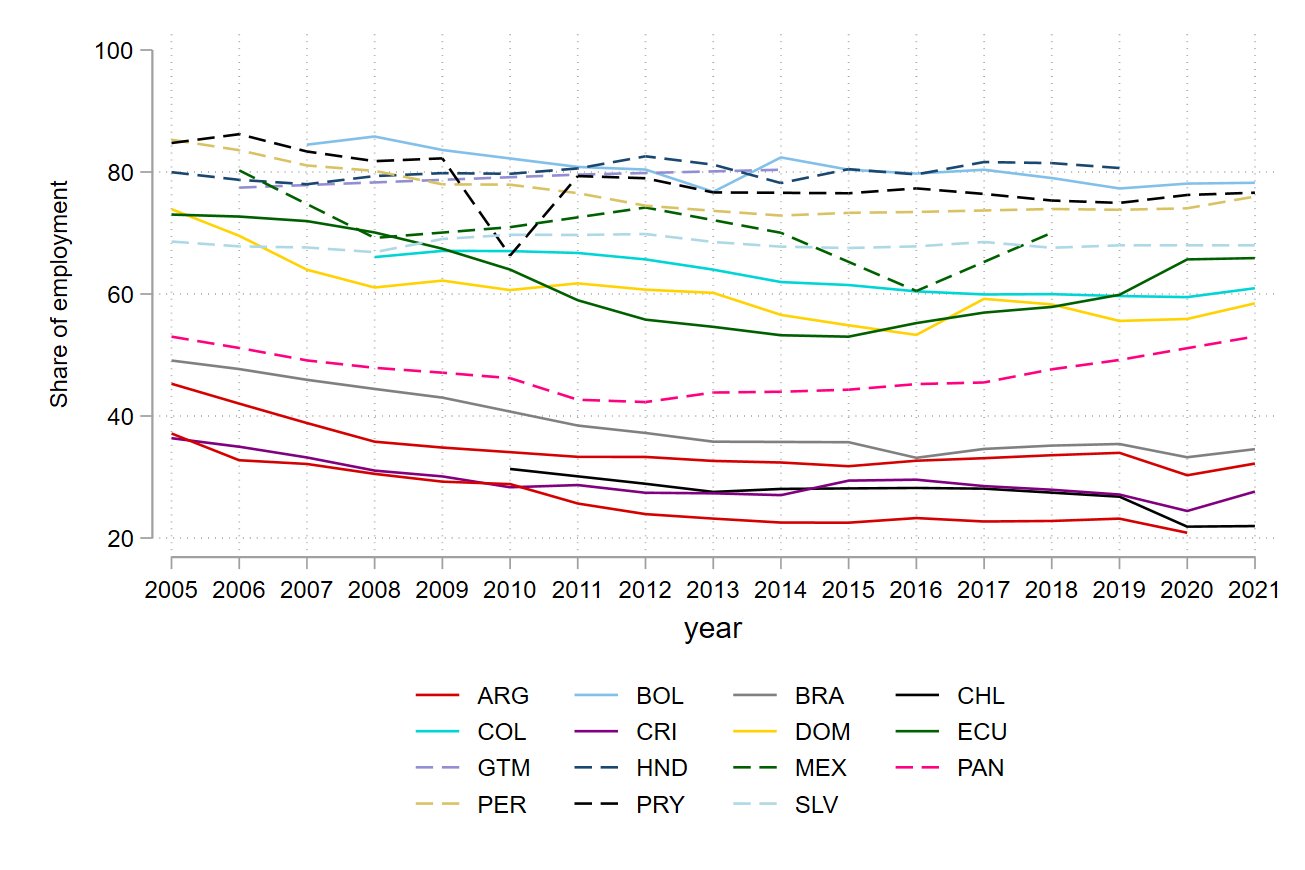
\includegraphics[scale=.2]{latex/figures/Evolution/informal_ss_all.png}
        \label{fig:Evolution_informalSS}
        \footnotesize{Source: Household Surveys-SEDLAC.}
       \footnotesize{Note SEDLAC: The figure shows unweighted means of country level indicators. The countries included in the sample are Argentina, Bolivia, Brazil, Chile, Colombia, Costa Rica, Ecuador, Guatemala, Dominican Republic, Honduras, Mexico, Panama, Peru, Paraguay, El Salvador and Uruguay. Some countries don’t have information for the entire period: Bolivia and Brazil have missing values in 2010; Colombia have missing values in 2006 and 2007; Honduras have missing values in 2020-2021; Mexico have missing values 2005, 2007, 2009, 2011, 2013, 2015, 2017, 2019, 2020, 2021; Panama and El Salvador have missing values 2020; and Uruguay have missing values in 2021.}
 \end{figure}
 \end{frame}
%---------------------------------------------------------
%---------------------------------------------------------
\begin{frame}
\frametitle{Dynamics: last 20 years}
\begin{figure}[!htb]
        \justifying
        \caption{Workers who are low skill self-employed or are employed at a small firm or zero wage workers by country}     
        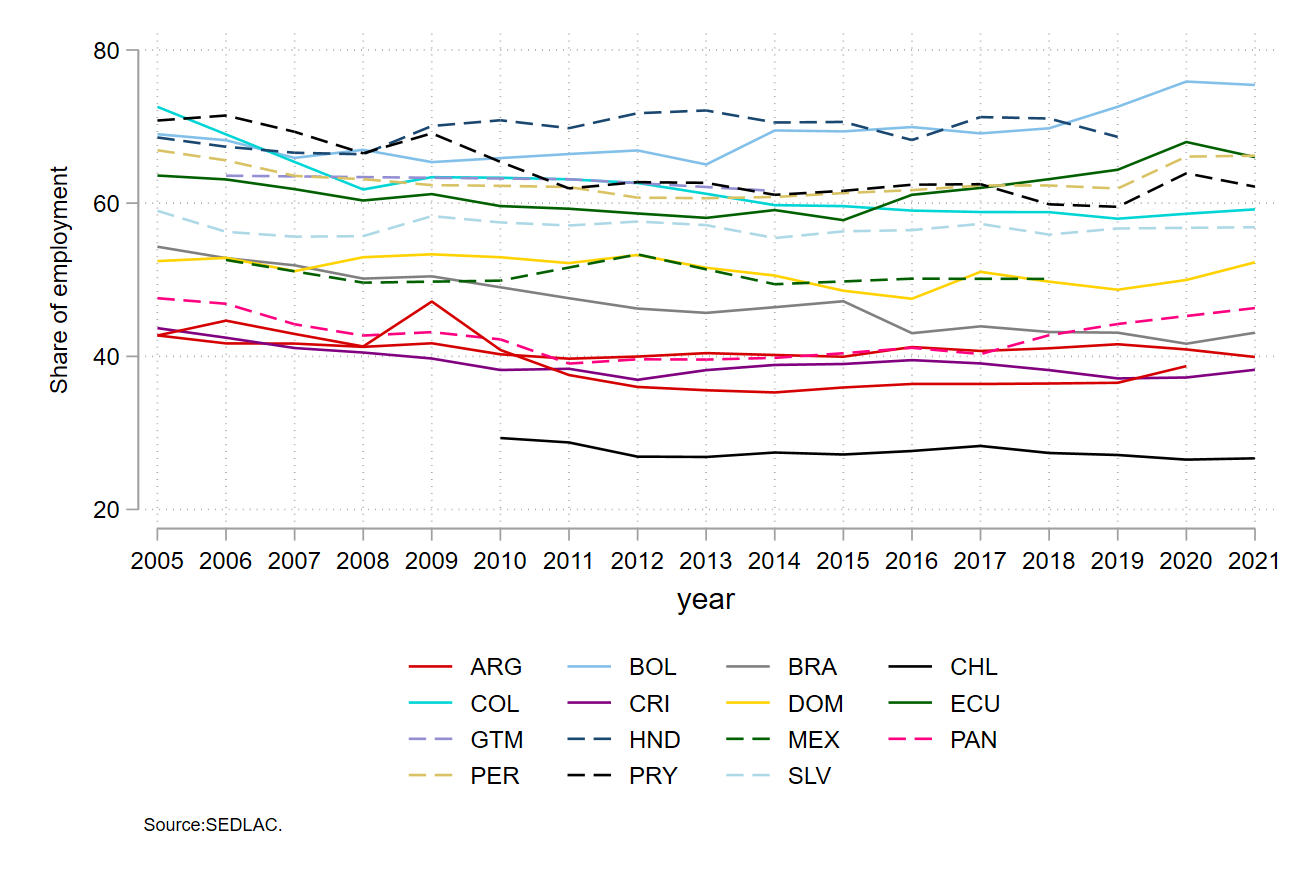
\includegraphics[scale=.2]{latex/figures/Evolution/informal_pr_all.png}
        \label{fig:Evolution_informalpr}
        \footnotesize{Source: Household Surveys-SEDLAC.}
       \footnotesize{Note SEDLAC: The figure shows unweighted means of country level indicators. The countries included in the sample are Argentina, Bolivia, Brazil, Chile, Colombia, Costa Rica, Ecuador, Guatemala, Dominican Republic, Honduras, Mexico, Panama, Peru, Paraguay, El Salvador and Uruguay. Some countries don’t have information for the entire period: Bolivia and Brazil have missing values in 2010; Colombia have missing values in 2006 and 2007; Honduras have missing values in 2020-2021; Mexico have missing values 2005, 2007, 2009, 2011, 2013, 2015, 2017, 2019, 2020, 2021; Panama and El Salvador have missing values 2020; and Uruguay have missing values in 2021.}
 \end{figure}
 \end{frame}
%---------------------------------------------------------
%---------------------------------------------------------
\begin{frame}
\frametitle{Dynamics: last 20 years}
\begin{figure}[!htb]
        \justifying
        \caption{Salaried workers who do not contribute to SS by country}     
        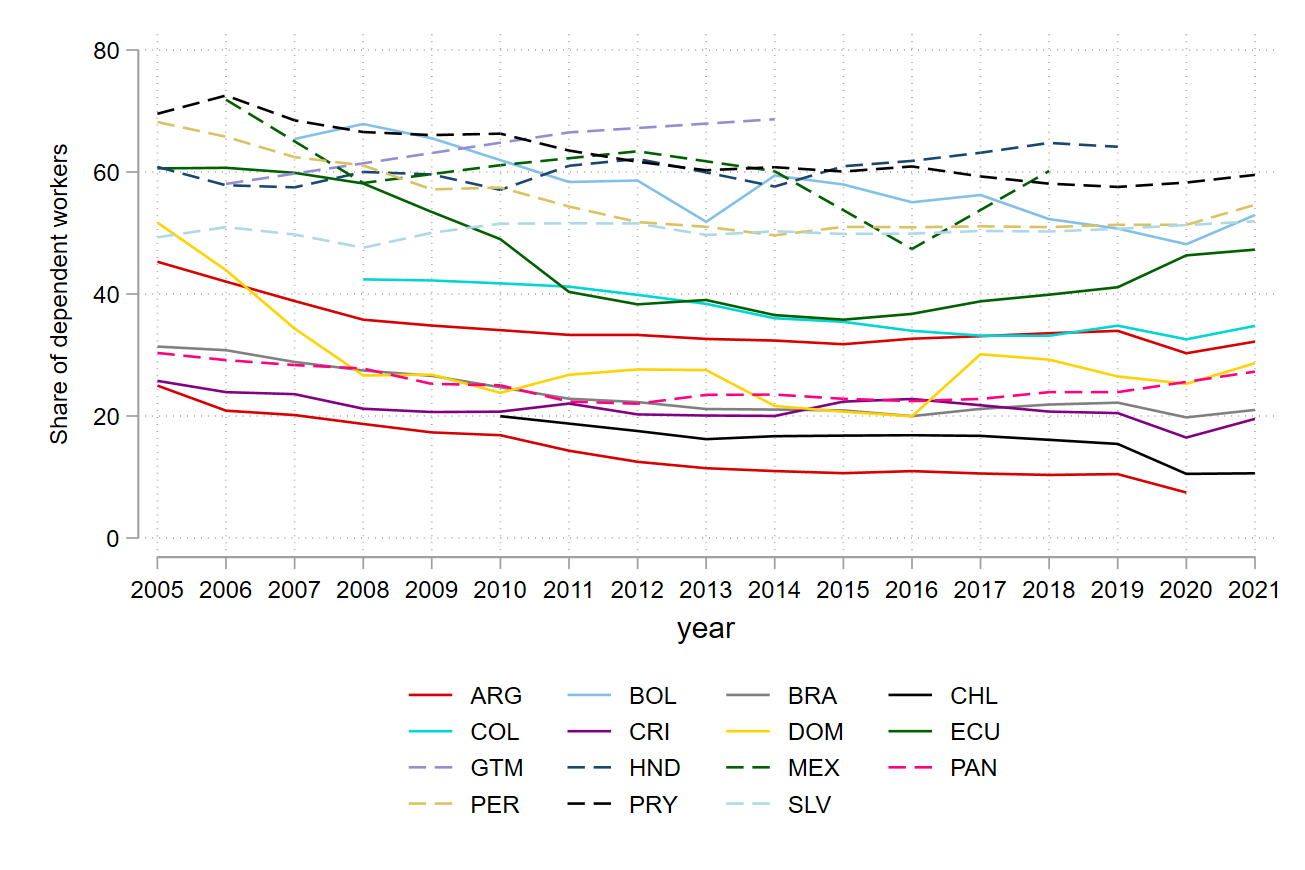
\includegraphics[scale=.2]{latex/figures/Evolution/informal_ss_dep_all.png}
        \label{fig:Evolution_informalssdep}
        \footnotesize{Source: Household Surveys-SEDLAC.}
       \footnotesize{Note SEDLAC: The figure shows unweighted means of country level indicators. The countries included in the sample are Argentina, Bolivia, Brazil, Chile, Colombia, Costa Rica, Ecuador, Guatemala, Dominican Republic, Honduras, Mexico, Panama, Peru, Paraguay, El Salvador and Uruguay. Some countries don’t have information for the entire period: Bolivia and Brazil have missing values in 2010; Colombia have missing values in 2006 and 2007; Honduras have missing values in 2020-2021; Mexico have missing values 2005, 2007, 2009, 2011, 2013, 2015, 2017, 2019, 2020, 2021; Panama and El Salvador have missing values 2020; and Uruguay have missing values in 2021.}
 \end{figure}
 \end{frame}
%--------------------------------------------------------
%-----------------------------------------------------------------------------------------------------------------
%--------------------------------------------------------
%---------------------------------------------------------
%---------------------------------------------------------
\begin{frame}
\frametitle{Dynamics: last 20 years}
\begin{figure}[!htb]
        \justifying
        \caption{Self-employed workers by country}     
        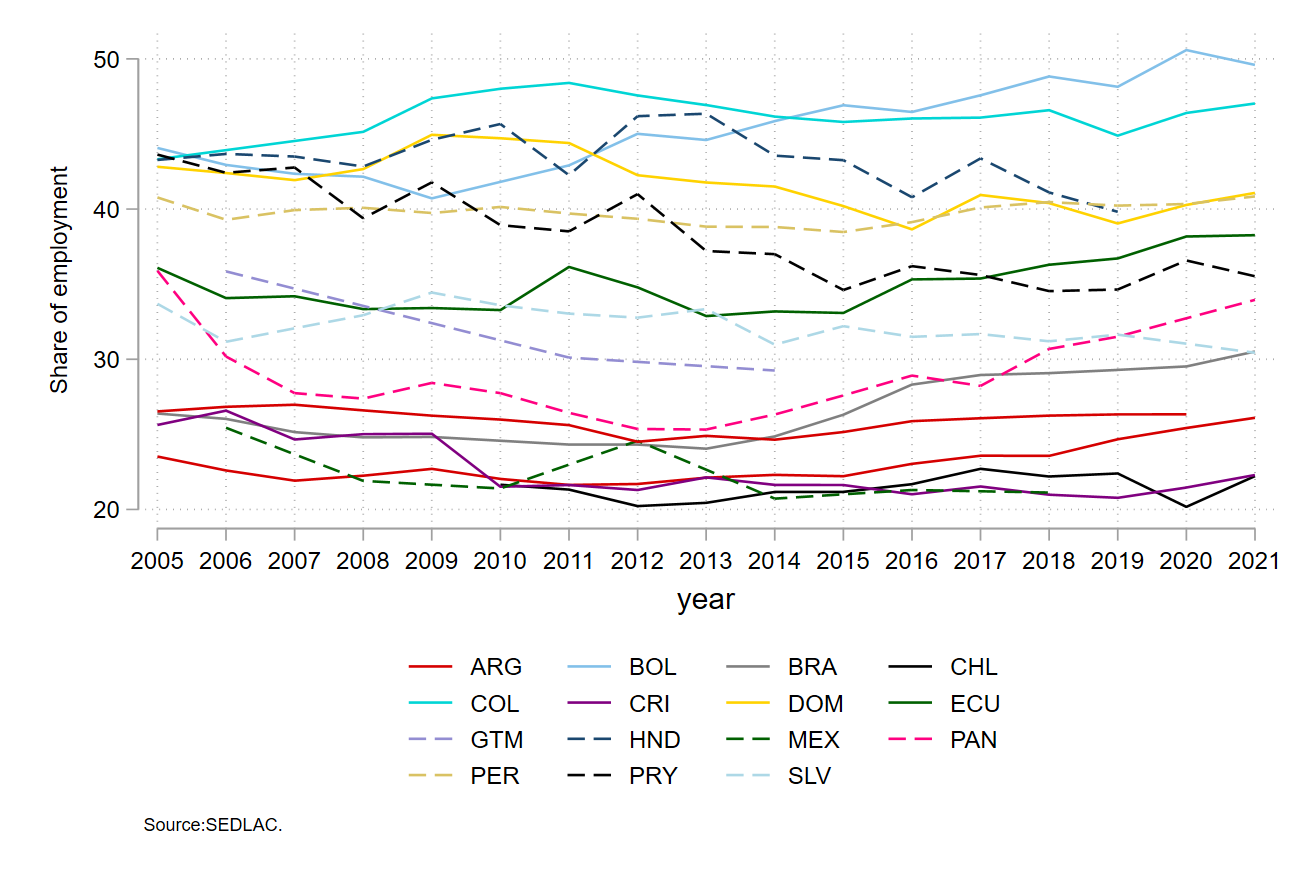
\includegraphics[scale=.2]{latex/figures/Evolution/self_employed_all.png}
        \label{fig:Evolution_selfemployed}
        \footnotesize{Source: Household Surveys-SEDLAC.}
       \footnotesize{Note SEDLAC: The figure shows unweighted means of country level indicators. The countries included in the sample are Argentina, Bolivia, Brazil, Chile, Colombia, Costa Rica, Ecuador, Guatemala, Dominican Republic, Honduras, Mexico, Panama, Peru, Paraguay, El Salvador and Uruguay. Some countries don’t have information for the entire period: Bolivia and Brazil have missing values in 2010; Colombia have missing values in 2006 and 2007; Honduras have missing values in 2020-2021; Mexico have missing values 2005, 2007, 2009, 2011, 2013, 2015, 2017, 2019, 2020, 2021; Panama and El Salvador have missing values 2020; and Uruguay have missing values in 2021.}
 \end{figure}
 \end{frame}
%---------------------------------------------------------
%---------------------------------------------------------
\begin{frame}
\frametitle{Dynamics: last 20 years}
\begin{figure}[!htb]
        \justifying
        \caption{Self-employed workers who do not contribute to SS by country}     
        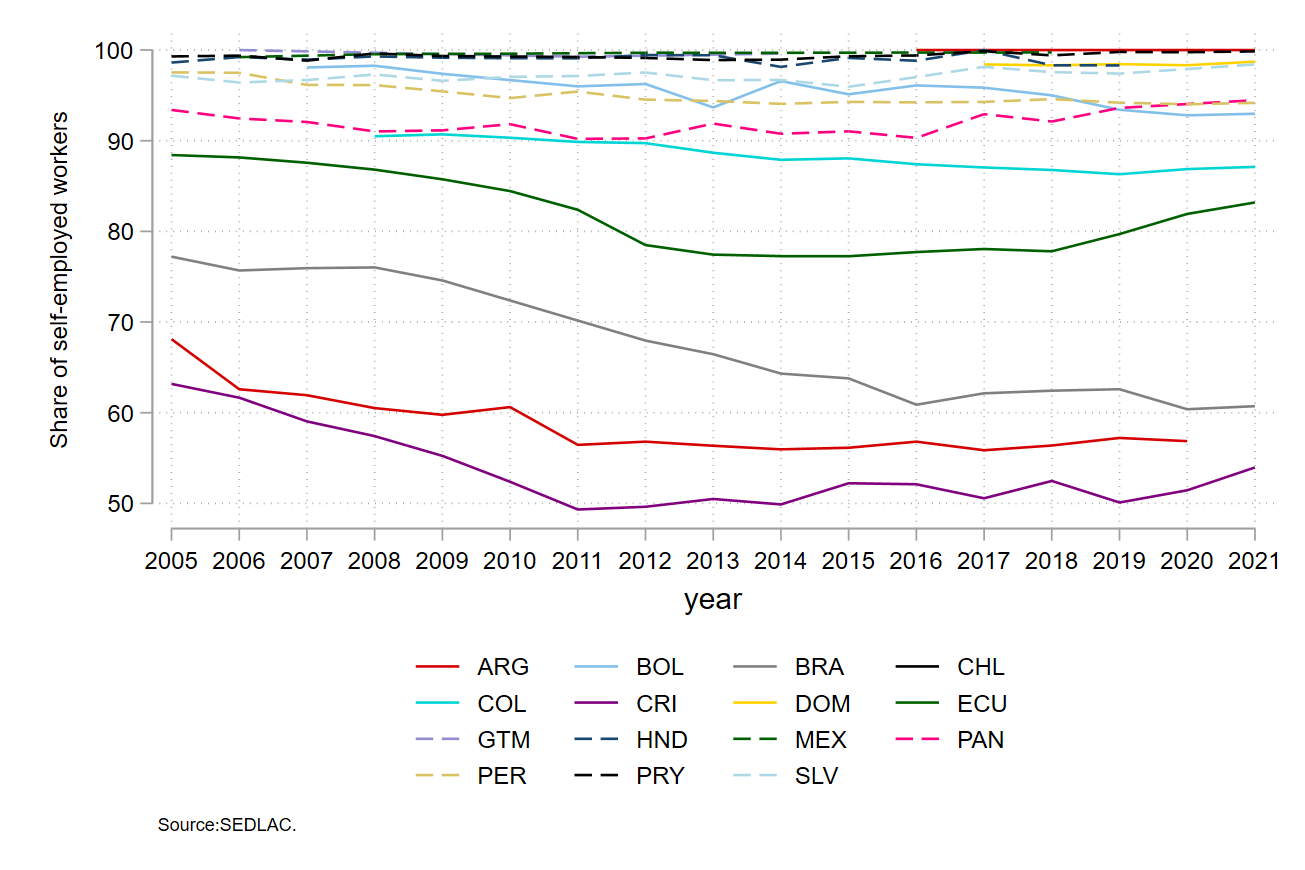
\includegraphics[scale=.2]{latex/figures/Evolution/iss_sfemployed_all.png}
        \label{fig:Evolution_selfemployedSS}
        \footnotesize{Source: Household Surveys-SEDLAC.}
       \footnotesize{Note SEDLAC: The figure shows unweighted means of country level indicators. The countries included in the sample are Argentina, Bolivia, Brazil, Chile, Colombia, Costa Rica, Ecuador, Guatemala, Dominican Republic, Honduras, Mexico, Panama, Peru, Paraguay, El Salvador and Uruguay. Some countries don’t have information for the entire period: Bolivia and Brazil have missing values in 2010; Colombia have missing values in 2006 and 2007; Honduras have missing values in 2020-2021; Mexico have missing values 2005, 2007, 2009, 2011, 2013, 2015, 2017, 2019, 2020, 2021; Panama and El Salvador have missing values 2020; and Uruguay have missing values in 2021.}
 \end{figure}
 \end{frame}
%--------------------------------------------------------
%--------------------------------------------------------
%---------------------------------------------------------
%---------------------------------------------------------
%---------------------------------------------------------
%---------------------------------------------------------
%---------------------------------------------------------
%---------------------------------------------------------
%---------------------------------------------------------
%---------------------------------------------------------
%---------------------------------------------------------
%---------------------------------------------------------
%---------------------------------------------------------
%---------------------------------------------------------
%---------------------------------------------------------
%---------------------------------------------------------
%---------------------------------------------------------
%---------------------------------------------------------
%---------------------------------------------------------
%---------------------------------------------------------
%---------------------------------------------------------


\end{document}